\fancyhf{}
\fancyfoot[CO, CE]{ \thepage}

\chapter{Prior work}
\label{chapter2}

\section{Literature survey}

The demand for efficient hardware accelerators, particularly deep learning applications, has grown rapidly. This has led to many frameworks being developed for generating specialized hardware with less human intervention. These frameworks utilize High-Level Synthesis, Intermediate Representations (IR), and other advanced optimizations to automate the design process from software algorithms to hardware implementation. This section compares state-of-the-art frameworks, including POLSCA \cite{POLSCA}, ScaleHLS \cite{DBLP:journals/corr/abs-2107-11673}, POM \cite{zhang2024optimizingframeworkmlirefficient}, and SODA \cite{BohmAgostini2022BridgingPT}. Comparison is made based on target platforms and optimization strategies.

\subsection{POLSCA}

POLSCA \cite{POLSCA} framework explores polybench kernels performance on HLS, with a primary focus on loop transformations to enhance the C++ code. Unlike SODA, it cannot take input from high-level languages like Python. This limits its flexibility in terms of usage in deep learning applications. The framework evaluates only polybench kernels and lacks performance analysis of neural networks.

\subsection{ScaleHLS}

ScaleHLS \cite{DBLP:journals/corr/abs-2107-11673} is a powerful framework that has finer control over the optimizations applied at different levels of abstraction including graph, loop and directive levels. Whilst this control is beneficial for FPGAs, it can introduce complexities while targeting ASICs. Very high levels of fine-tuning can be impractical considering the high cost of iterative design cycles in ASICs. ScaleHLS lacks layer-by-layer analysis of neural networks that SODA can offer. Another limitation of ScaleHLS is that it needs to be annotated back to HLS C code. By applying optimizations at lower level of abstraction and subsequently raising the abstraction level can lead to loss of performance potentially. In contrast, SODA doesn't need to be converted back to HLS C, this preserves all the optimizations applied at lower levels of abstraction, making it more suitable for ASIC and FPGA designs.

\subsection{POM}

The POM \cite{zhang2024optimizingframeworkmlirefficient} framework focuses on FPGA-based accelerators along with MLIR optimizations. It employs advanced dependency analysis in MLIR to maximize FPGA specific optimizations. The framework works well with large-scale deep learning models, achieving significant improvements with loop optimizations and pipelining strategies. Layer-by-layer analysis of deep learning models is also shown. But the problem with this is that as layer size increases, the resources utilized in FPGA increases as well. This is a problem when targeting ASICs. Consequently, SODA layer-by-layer analysis must adapt to accurate resource allocation to control the ASIC's power, performance, and area (PPA) metrics.

\subsection{SODA}

The SODA framework stands out by supporting both FPGA and ASIC synthesis, making it more versatile compared to frameworks like ScaleHLS, POLSCA, and POM, which are primarily FPGA-focused. Built on MLIR, SODA automates the end-to-end process of hardware generation from high-level frameworks such as TensorFlow and PyTorch, requiring minimal manual intervention. This automation is particularly beneficial for ASIC designs, where manually writing RTL code is time-consuming and error-prone. SODA allow users to evaluate various trade-offs between power, performance, and area (PPA) enabling optimal hardware designs.

\subsubsection{Python to ASIC (Application Specific Integrated Circuit) Flow}

\begin{figure}[H]
    \centering
    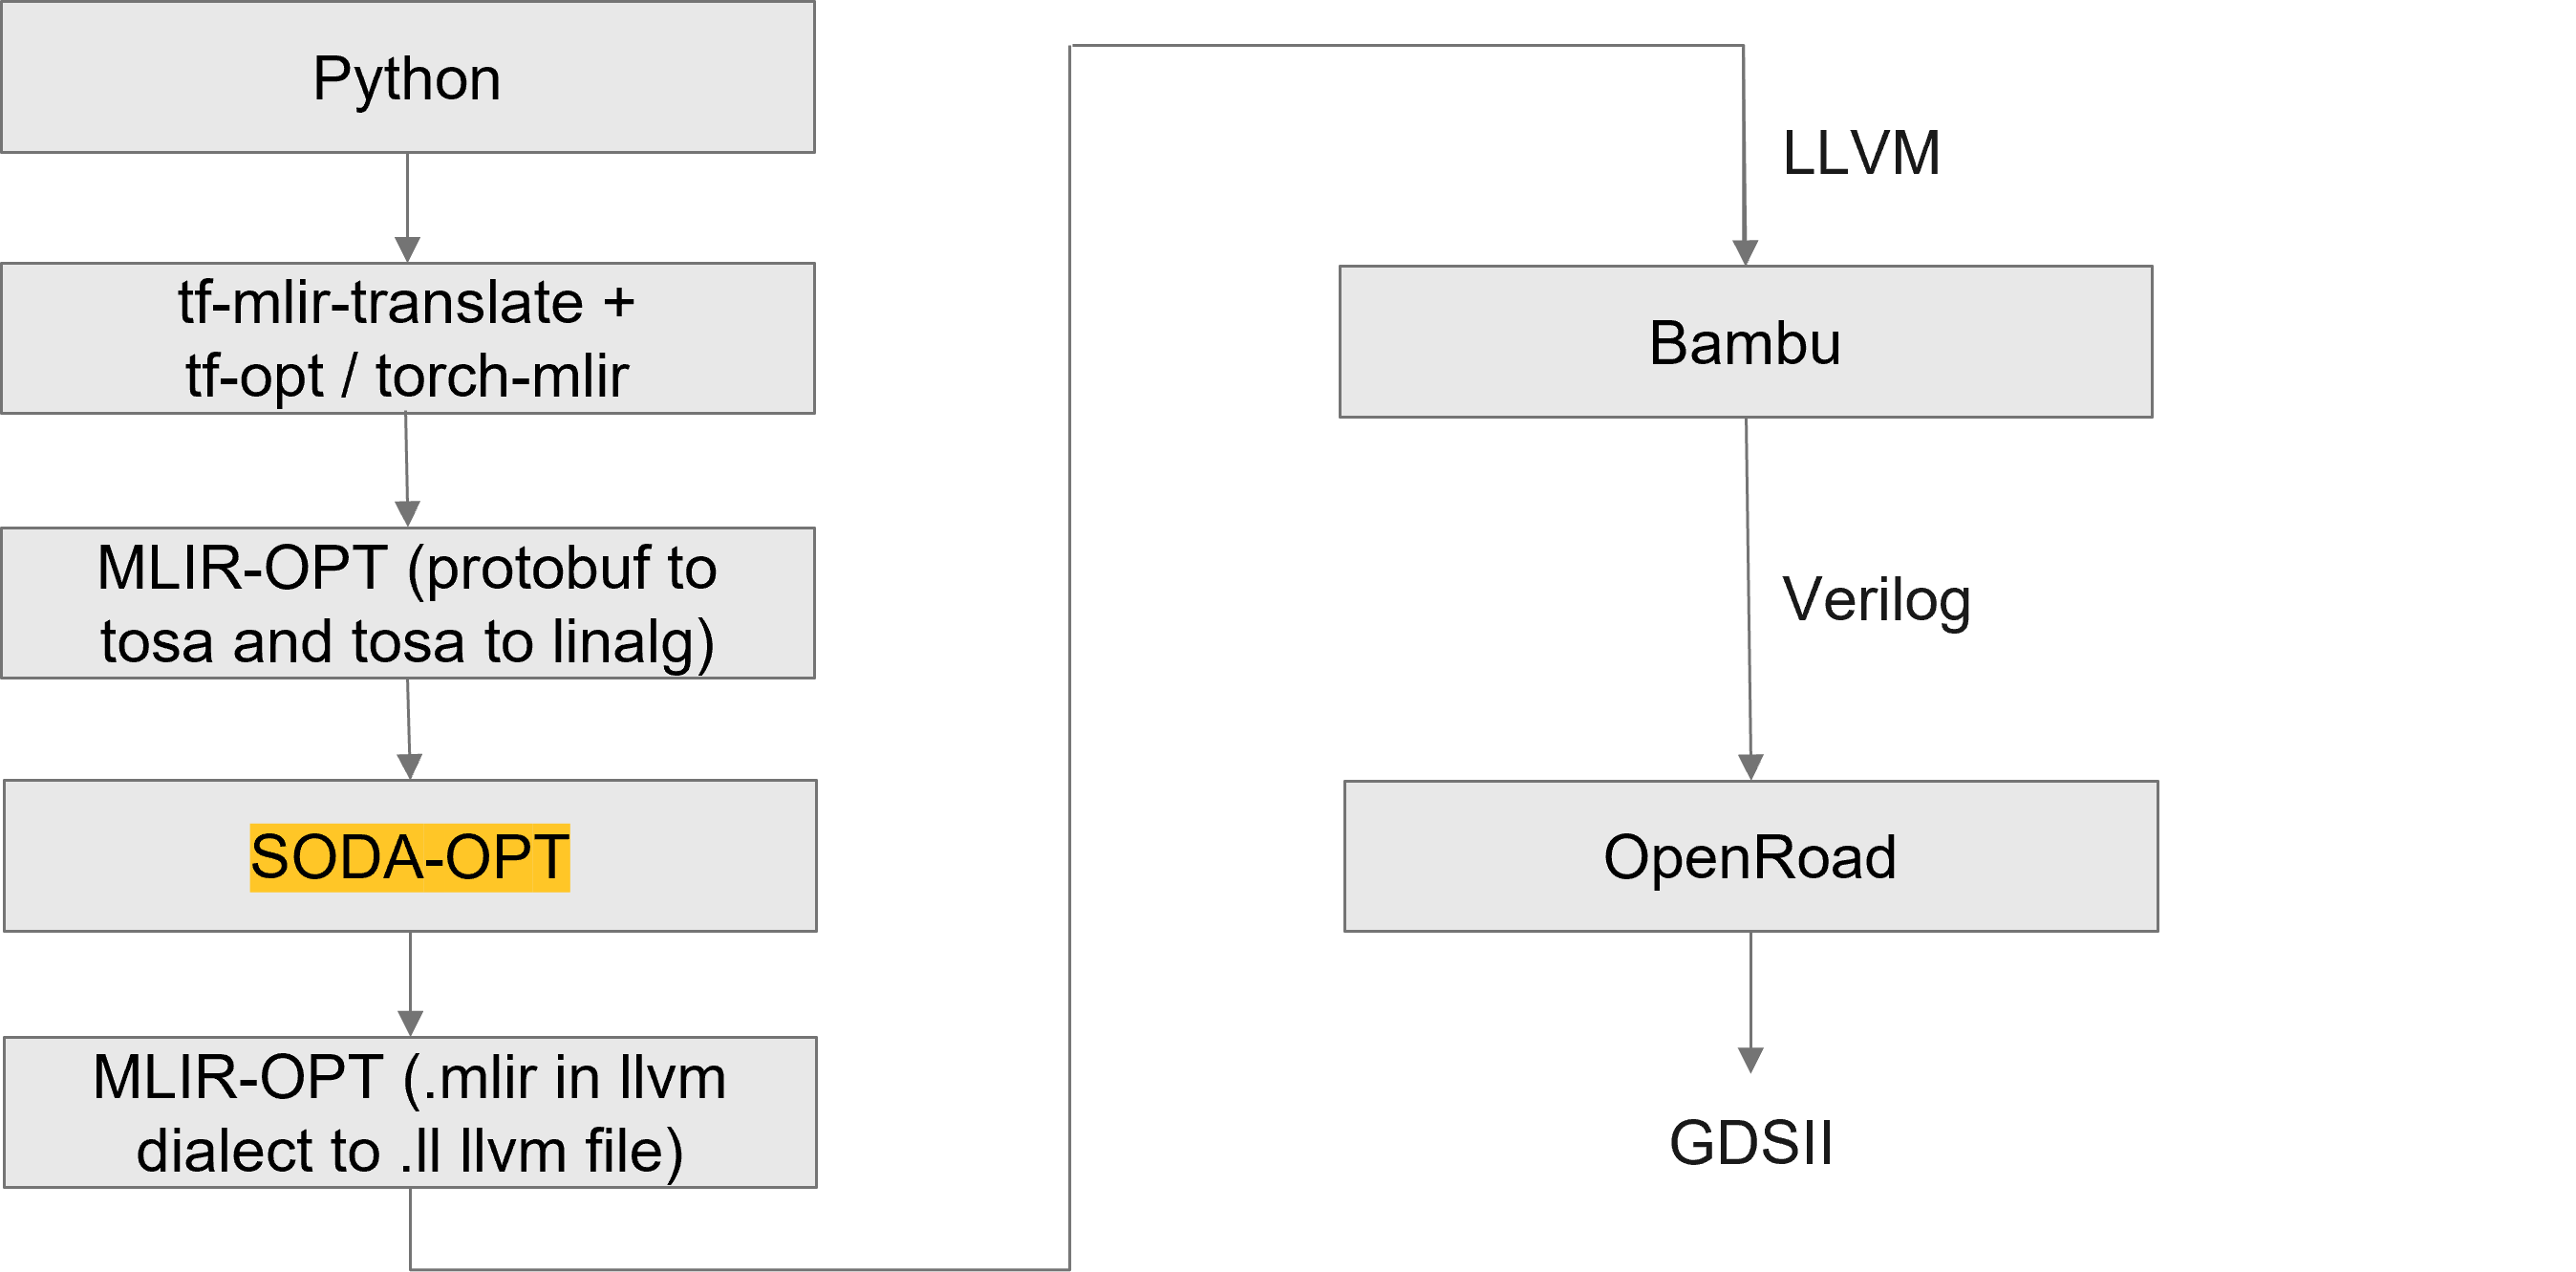
\includegraphics[width=0.8\linewidth]{figure//chapter1_intro/Fig 1 - Python to ASIC flow.png}
    \caption{Python to ASIC flow}
    \label{fig:1.1}
\end{figure}

Synthesizing Python based deep learning models into an ASIC involves multiple steps. Here is the description of the steps:

\begin{enumerate}
    
    \item Python: The flow begins with deep learning models described in Python, typically using frameworks like TensorFlow or PyTorch.

    \item Translating Python to MLIR: The Python code is translated into MLIR (Multi-Level Intermediate Representation) format. TensorFlow models are processed using tf-mlir-translate and tf-opt, while PyTorch models use torch-mlir.

    \item MLIR-OPT (converts Protobuf to Linalg): The translated MLIR code is further optimized by converting TensorFlow operations (protobuf) to the TensorFlow Lite TOSA (Tensor Operation Set Architecture) format, followed by a conversion to Linalg (linear algebra operations) dialect in MLIR.

    \item SODA: At this stage, SODA partitions host code and accelerated code. Applies loop optimizations and memory optimizations for the accelerated code to generate ASIC for this particular layer of neural network.

    \item MLIR-OPT (converts .mlir file to .ll file): After applying all the optimizations, the MLIR is converted into LLVM dialect and further into an LLVM intermediate file (.ll), prepared to be synthesized.

    \item Bambu: The LLVM code is processed by the Bambu HLS tool, which translates the intermediate code into Verilog for hardware synthesis.

    \item OpenRoad: The Verilog code is then used by OpenRoad, an open-source physical design tool, to generate the final GDSII (Graphical Data Stream Information Interchange) file used in ASIC manufacturing.
    
\end{enumerate}


\subsubsection{SODA}

\begin{figure}[H]
    \centering
    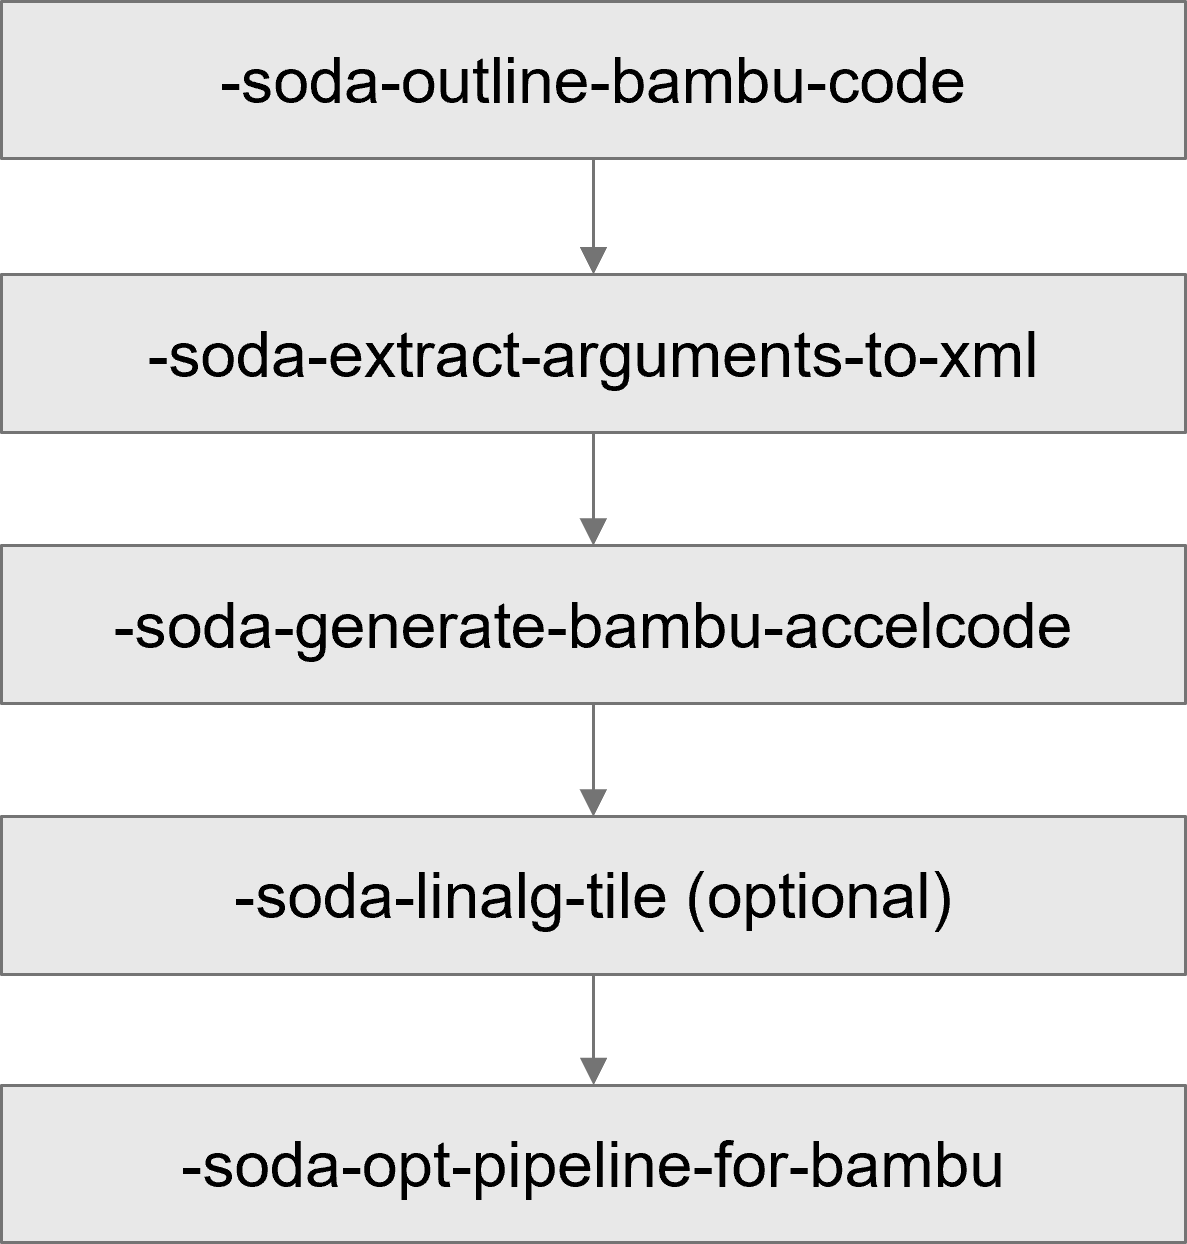
\includegraphics[width=0.4\linewidth]{figure//chapter1_intro/Fig 2 - SODA-OPT Flow.png}
    \caption{SODA flow}
    \label{fig:1.2}
\end{figure}

SODA framework has multiple passes to be executed to isolate accelerated code before applying optimizations. These passes are:

\begin{enumerate}
    
    \item -soda-outline-bambu-code: This pass isolates the host code from accelerated code. Accelerated code is outlined into separate kernel functions.
    \item -soda-extract-arguments-to-xml: In this step, the inputs and the output structure is extracted into an XML file. An XML file with initial values for the port is also generated. 
    \item -soda-generate-bambu-accelcode: After the code has been outlined into Bambu-compatible kernel functions, this step extracts them into individual, simplified MLIR modules.
    \item -soda-linalg-tile (optional): This step, performans tiling at linalg dialect. This helps with producing smaller ASICs for the same neural network layer.
    \item -soda-pipeline-for-bambu: This pass runs the full optimization pipeline to prepare the outlined accelerated code for Bambu.

\end{enumerate}

\subsubsection{Dialects utilized in SODA pipeline for Bambu:}

\begin{enumerate}
    
    \item Linalg dialect: It provides operations like `linalg.matmul`, `linalg.conv`, and more, which encapsulate common linear algebra routines. These operations are often used in high-performance computing, deep learning, and other domains where matrix and tensor computations are central.

    \item Affine dialect: Represents affine loops and memory accesses, providing a foundation for loop optimizations and transformations.

    \item Structured Control Flow (SCF) dialect: Provides structured control flow operations like loops and conditionals, enabling high-level representation of control flow in MLIR.

    \item Control Flow (CF) dialect: Implements unstructured control flow primitives, such as branches and jumps, allowing fine-grained control over program execution paths.
    
    \item Low-Level Virtual Machine (LLVM) dialect: Represents low-level operations and constructs directly compatible with the LLVM IR, facilitating the transition from MLIR to LLVM-based code generation.
    
\end{enumerate}

\subsubsection{SODA pipeline for Bambu:}

\begin{figure}[H]
    \centering
    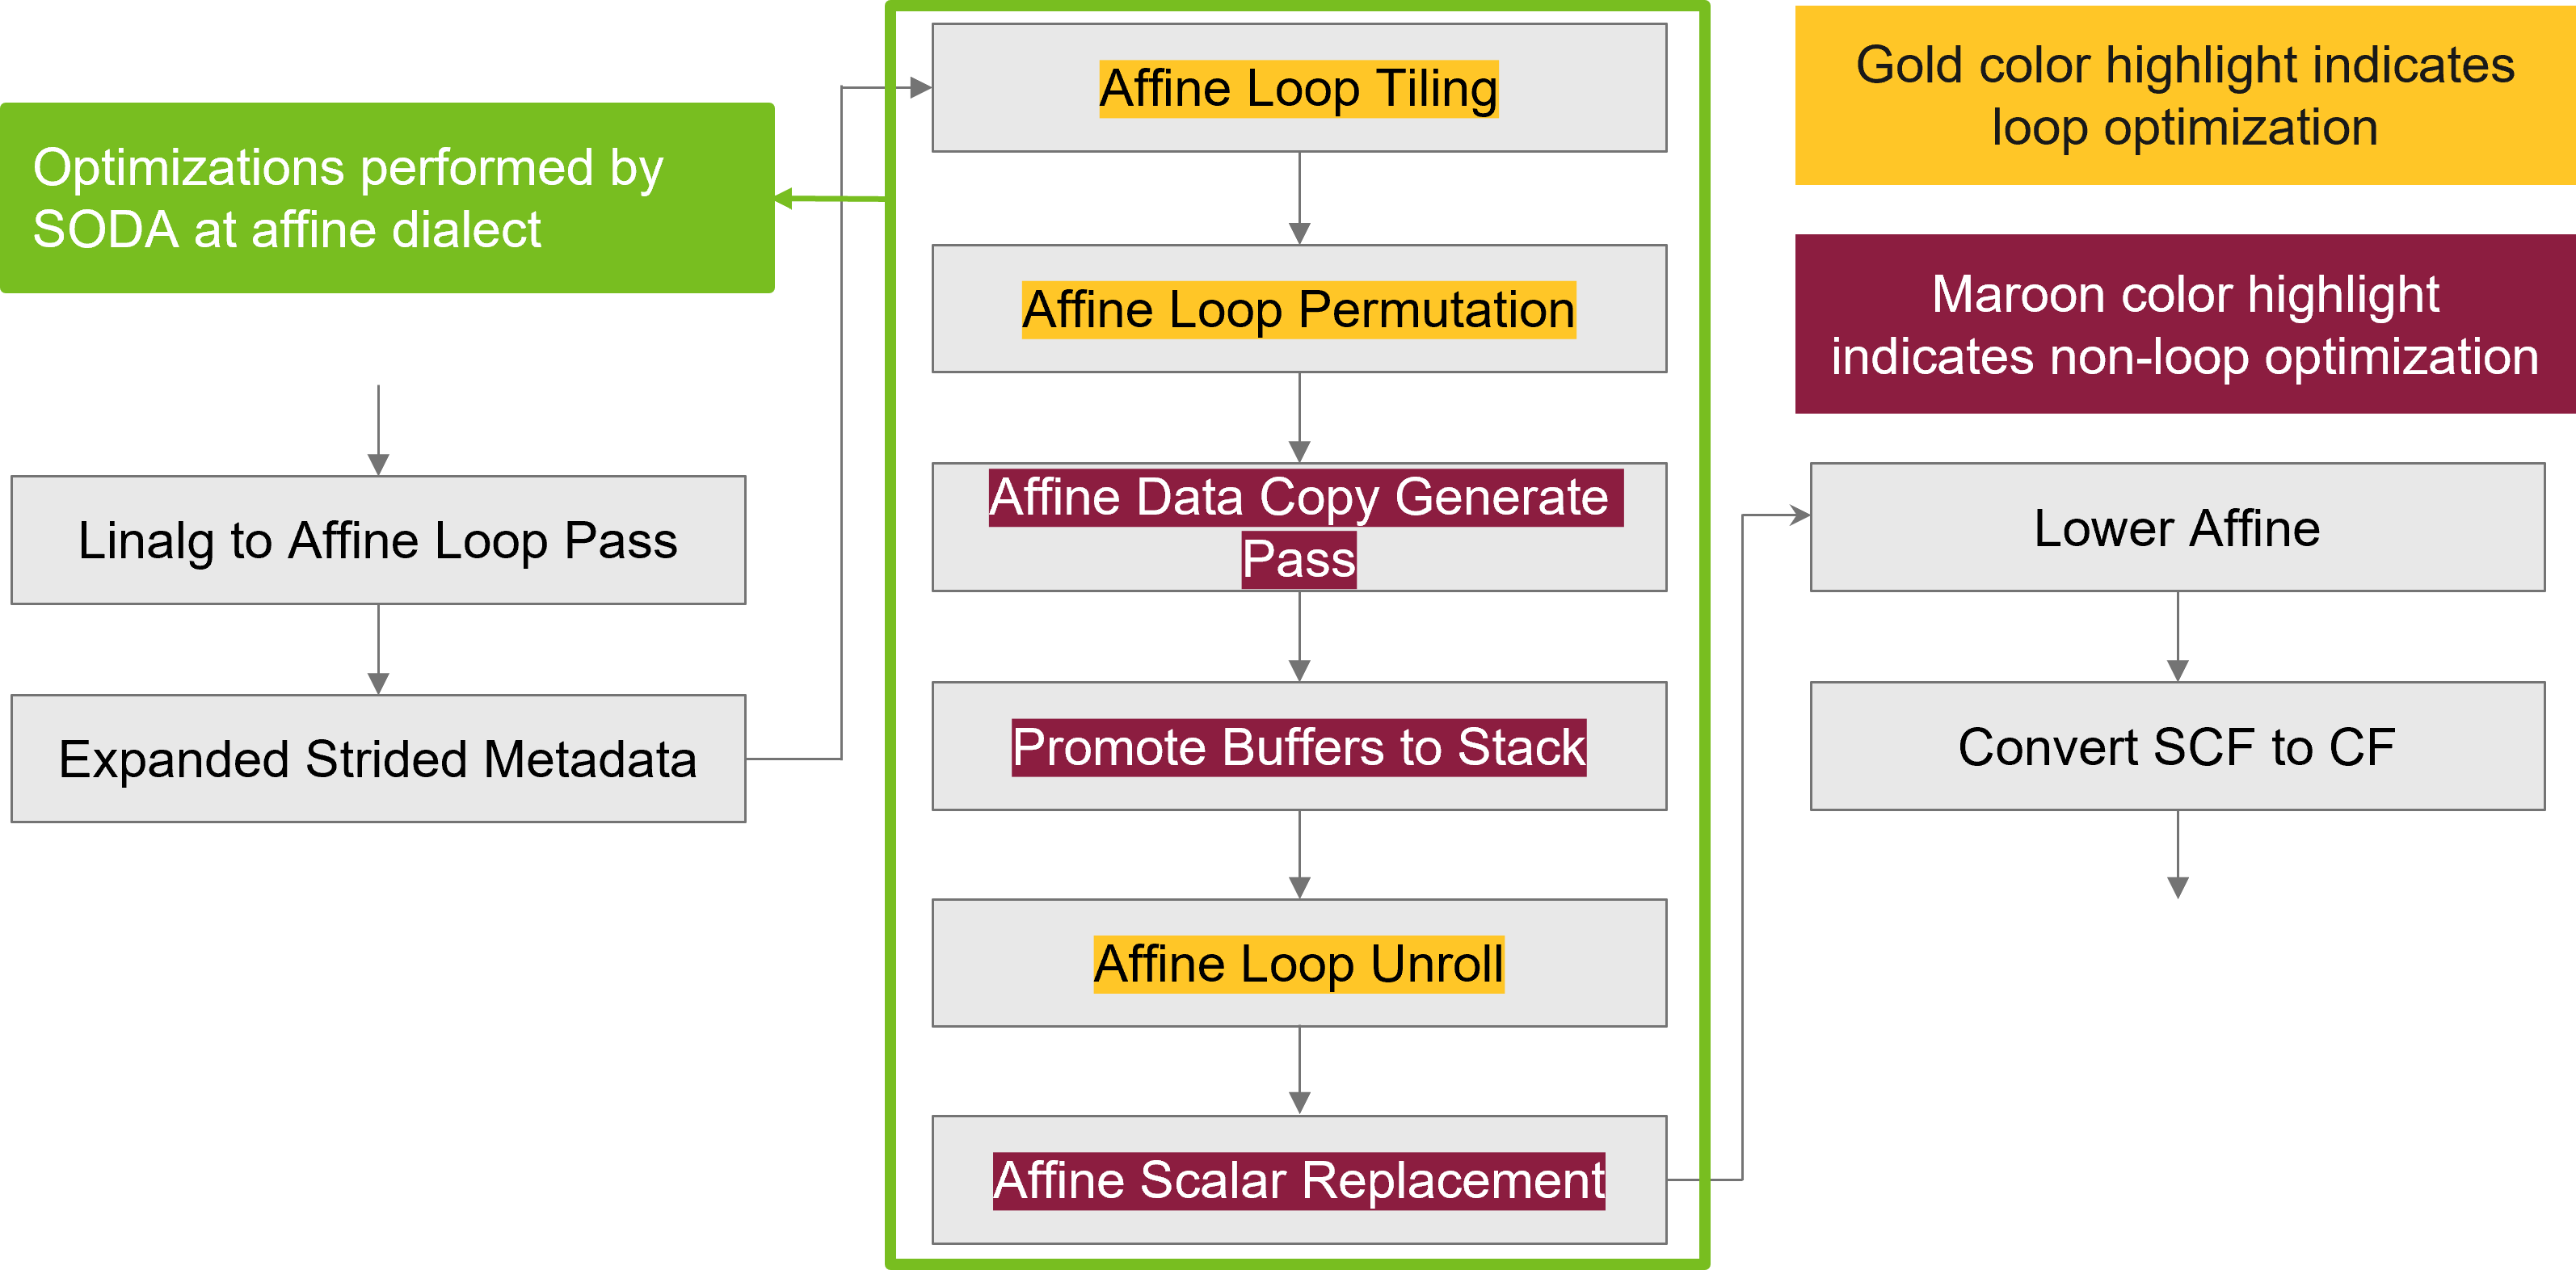
\includegraphics[width=1\linewidth]{figure//chapter1_intro/Fig 3 - Pipeline for Bambu.png}
    \caption{SODA Pipeline for Bambu flow (Linalg dialect to CF dialect)}
    \label{fig:1.3)}
\end{figure}

AS shown in Figure 1.3, within the '\textit{-soda-pipeline-for-bambu}' pass, the accelerated code at Linalg level is lowered to Affine level dialect. SODA now applies the required loop optimizations and other optimizations required to enhance the accelerated code. After applying optimizations, the Affine level code is converted to SCF dialect and then converted to CF dialect.  

\begin{figure}
    \centering
    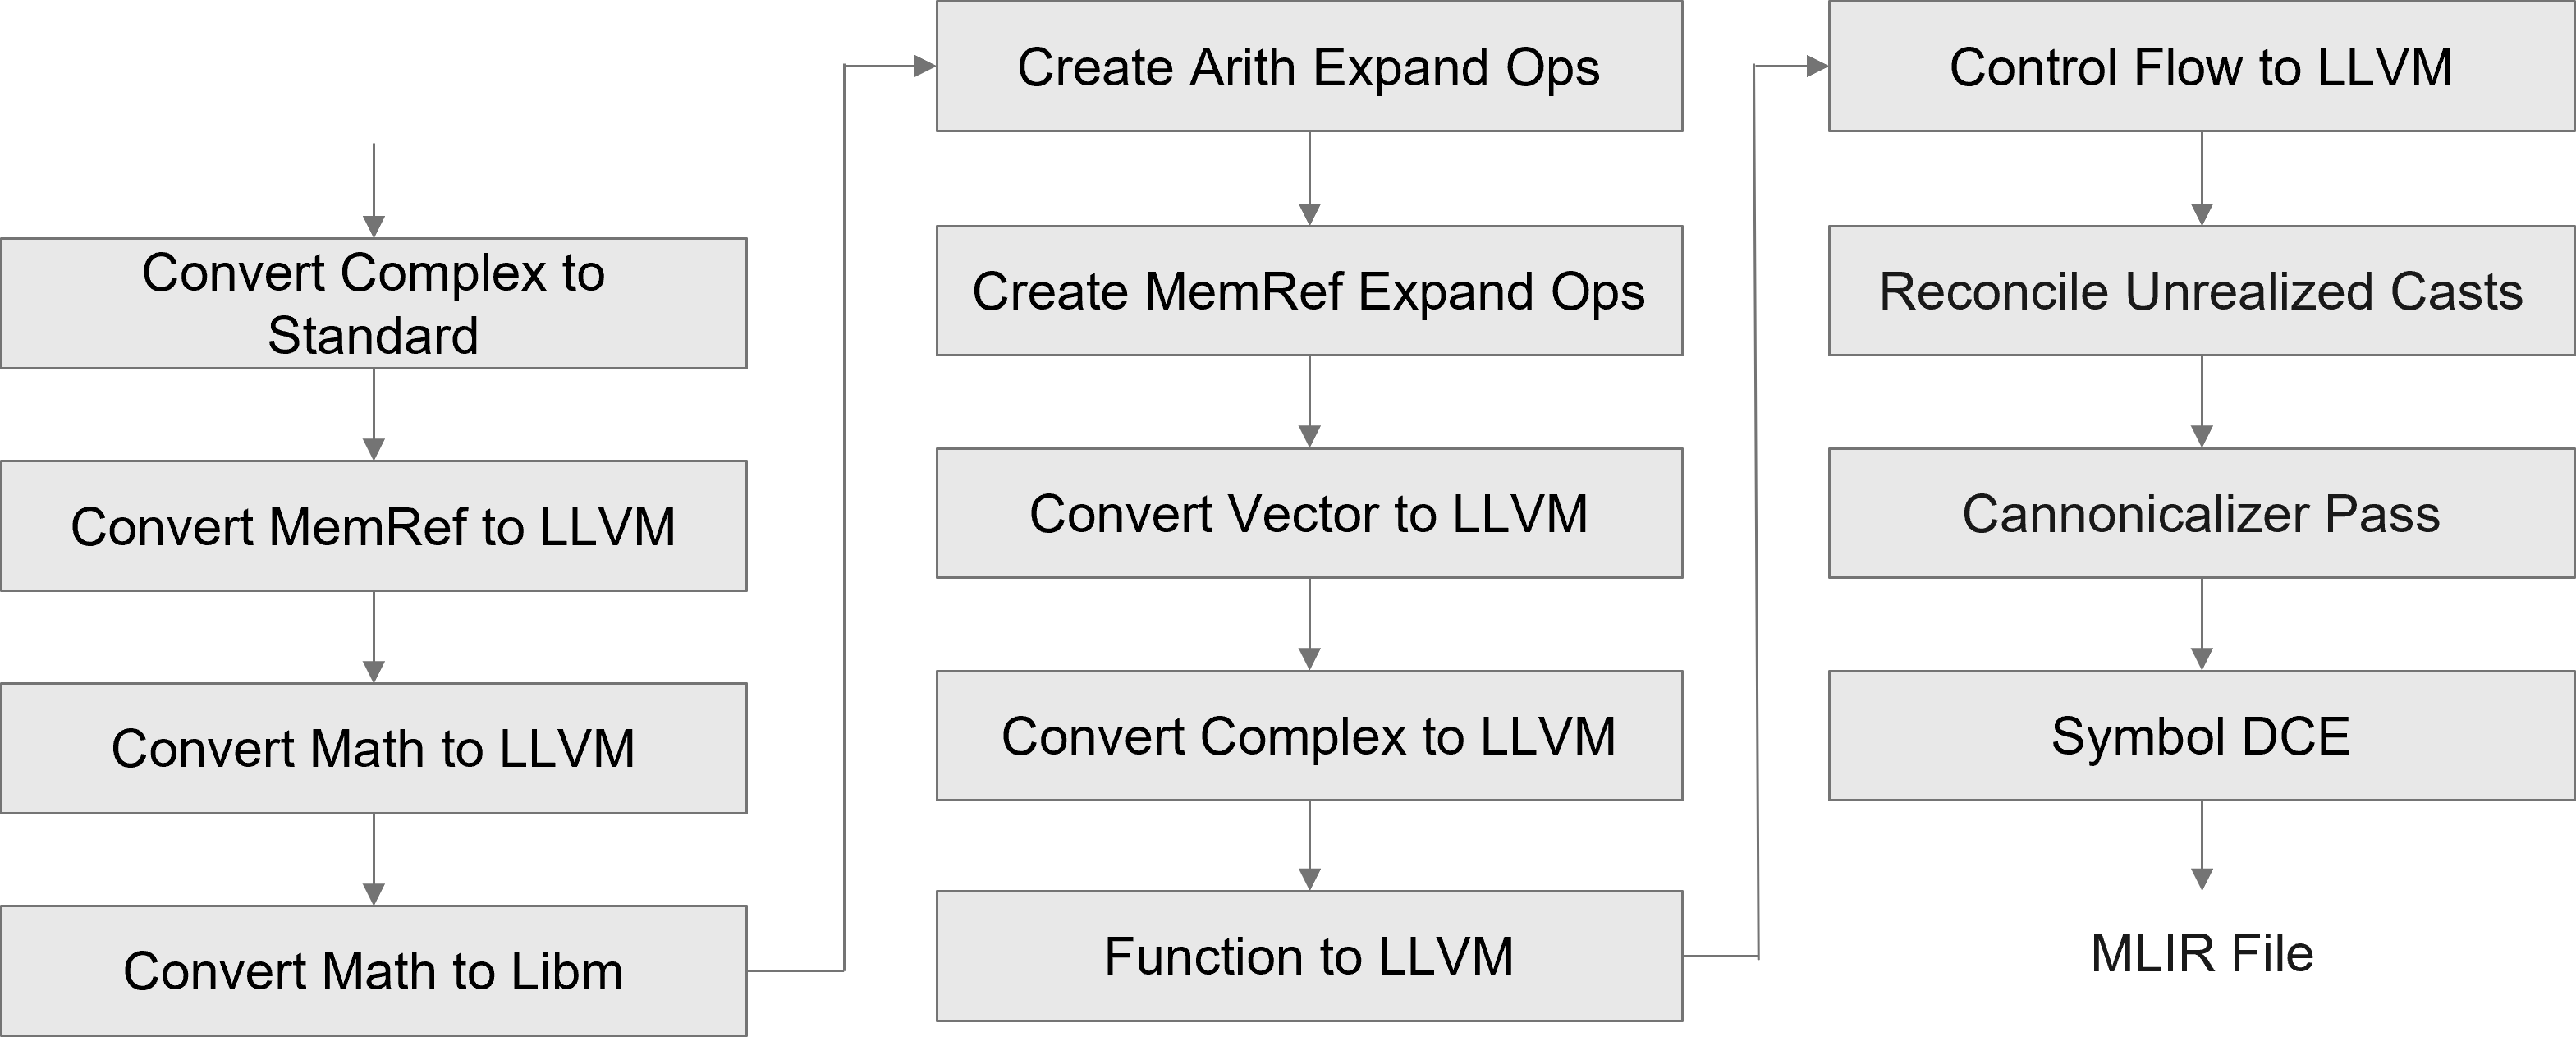
\includegraphics[width=0.9\linewidth]{figure//chapter1_intro/Fig 4 - Pipeline for Bambu 2.png}
    \caption{SODA Pipeline for Bambu flow (CF dialect to LLVM Dialect)}
    \label{fig:1.4)}
\end{figure}

Additional passes are added in the end to convert to LLVM dialect. The resulting MLIR file generated has the accelerated code encapsulated within an MLIR module in LLVM dialect. The flow is shown in Figure 1.4.

\subsubsection{Limitations of SODA framework}

\begin{table}[H]
\centering
\caption{SODA framework limitations and remarks}
\renewcommand{\arraystretch}{1.2} % Adjust row height
\small % Reduce font size
\resizebox{\textwidth}{!}{%
\begin{tabular}{|p{3cm}|p{4cm}|p{8cm}|}
\hline
\textbf{Tool} & \textbf{Limitations} & \textbf{Remarks} \\ \hline
\multirow{5}{*}{SODA} 
& Loop permutation& 1) Cannot give permutation order.\\
 & &2) Loop permutation pass doesn't map correctly.\\ \cline{2-3} 
& Loop tiling& 1) Only one uniform tile size can be given.\\
 & &2) Promote buffers to stack doesn't work with tiling.\\ \cline{2-3} 
& Loop unrolling & 1) Explores the option of fully unrolled loops only.\\
 & &2) SODA pipeline for Bambu gets stuck at Affine scalar replacement.\\
 & &3) Unrolling generates too many flip-flops.\\ \hline
\multirow{1}{*}{Bambu} 
& Simulation clock cycles limit & Bambu generates a testbench that has clock cycles limit on how long testbench can be run for. If the design takes longer than the simulation limit, it fails to synthesize larger neural networks to a chip. \\ \hline
\multirow{1}{*}{Yosys (OpenRoad)} 
& BRAM synthesis & Yosys synthesis tool in OpenRoad fails to synthesize BRAM module for larger neural networks. \\ \hline
\end{tabular}
}
\end{table}

The Table 2.1 summarizes the limitations in SODA, Bambu and Yosys tools. 

The SODA framework mainly has loop optimization issues related to loop permutation, loop tiling, and loop unrolling. 
\begin{itemize}
    \item Loop permutation: In the case of loop permutation, the SODA pipeline for Bambu includes a pass to take in the permutation order, but that does not function as intended. Additionally, the test loop permutation in MLIR-OPT does not consistently map the permutations correctly for all permutations. This limitation affects the cases where loop permutation could lead to significant performance improvements.

    \item Loop tiling: The tiling option in SODA pipeline for Bambu takes only one value of tile size for all the nested for-loops. This is a disadvantage in terms of testing out different tile sizes, to get the best tiling combination. Furthermore, promote buffers to stack memory optimization doesn't work along with tiling.

    \item Loop unrolling: In this optimization, only the option of completely unrolling the loop is explored. However, loops can be unrolled partially by a factor. This could yield better PPA. The second problem is that scalar replacement after unrolling results in taking the pass too long to execute, as unrolling would result in lots of scalars to be replaced. The third problem is that unrolling generates too many flip-flops as the body of the nested for loop is expanded. This causes hindrance to synthesize the design to an ASIC.
\end{itemize}

Bambu generates a test-bench from the XML file that contains input/output information. This generated test-bench has a limit on how many clock cycles it can be executed for. If the design under test exceeds this limit, it will fail to synthesize to an ASIC. This is a major area of concern to synthesize larger neural networks.

Yosys synthesis tool, integrated in OpenRoad tool, may find it difficult to synthesize designs that include Block-RAM (BRAM), particularly when the memory size is large. In general, memory is not synthesized using synthesis tools. Memory circuits are generated using memory compilers. This approach is necessary because often the synthesis tools struggle to meet the stringent timing constraints associated with memory synthesis.

Moreover, the paper \cite{BohmAgostini2022BridgingPT} presents results for a smaller neural architecture, such as LeNet-5, and focuses on relatively small layers of depth-wise convolution layers in MobileNet-V2. However, its application to larger neural network layers remains unexplored, limiting the understanding of its scalability and effectiveness in handling complex, real-world models.

\section{Research goals}

After a thorough evaluation of the limitations inherent to the SODA framework, the following research objectives have been identified.

\begin{enumerate}
    
    \item Address loop optimization challenges: Loop optimization plays a critical role in hardware synthesis, particularly for compute intensive operations in like neural networks. Managing loop permutation, loop tiling and loop unrolling to maximizes performance while keeping lowe resource utilization is critical when considering the cost of fabricating an ASIC.

    \item Explore methods to synthesize larger neural networks: Modern day neural architectures for computer vision and natural language processing demands significant compute resources. However, the inherent cost of manufacturing ASIC is very high. Therefore, we need to explore innovative techniques to efficiently synthesize large neural networks. This is a critical factor for scalability and efficiency of the framework.
    
    \item Design Space Exploration (DSE): This process entails systematically applying loop and memory optimizations to each layer of the neural network architecture, while also generating a customized set of optimizations tailored to the specific characteristics of each layer. Next step is to  generate the dataset for every layer.

    \item Analyzing results and identifying heuristics: Following the DSE and the dataset generation, the goal is to thoroughly investigate the PPA along with efficiency and energy consumed by the ASIC. Through this analysis of results, the aim is to narrow down the exploration space based on optimization applied and neural network layer characteristics, in order to reach the best performing ASIC at every layer.
    
\end{enumerate}

